% questions.tex —— 1977 年·江苏徐州市、徐州地区初试卷 · 题目内容片段（无答案）
% 由 tools/generate_projects.py 依来源总账自 1977/1977_数学真题_江苏徐州市,徐州地区初试_试题.md 生成，勿手改（改源 MD 后重跑）


\gkpart{江苏徐州市,徐州地区初试卷}

\begin{gktip}
\textbf{来源说明}：本题面依据固定源 PDF《1977江苏徐州市,徐州地区初试》第 1—2 页逐题转录。该 PDF 为 1977 年初试（预选）试卷编排本的扫描件，共 2 页：第 1 页为标题行与第一、二题（原书页码 241），第 2 页为第三至第十题（原书页码 242）。H1「七、徐州市、徐州地区」系原卷标题行逐字转写，其中「七、」为原书的地区序号而非题号。原卷题号为中文数字（一、二、……、十），本库按规范转写为阿拉伯数字题号；各题分值附记于题号之后，五道 8 分、三道 12 分、一道 14 分、一道 10 分，合计 100 分。原卷未附答案，配套答案与解析为本库编者独立推导，\textbf{非官方标准答案}。原卷无附加题与参考题。第 6、7 题右侧有原卷插图，第 9 题要求考生自绘图形。
\end{gktip}

\par\medskip

\begin{question}
\gkti{1}\textbf{（8 分）} 计算：

\nopagebreak[4]
\[
(-16)\div\left(-2\frac{2}{3}\right)^2+\left(\frac{1}{3}\right)^{-2}\times\left(\frac{3}{8}\right)^0-\left(\frac{9}{16}\right)^{\frac{1}{2}}.
\]

\end{question}
\begin{question}
\gkti{2}\textbf{（8 分）} 

（1） 把 $\dfrac{1}{\sqrt{3}-2}$ 的分母有理化；

（2） 已知 $x=\sqrt{2}+1$，求 $x^2-2x+1$ 的值。

\end{question}
\begin{question}
\gkti{3}\textbf{（8 分）} 求下列三角函数值：

（1） $\cos150^\circ$；

（2） $\operatorname{tg}\left(-\dfrac{\pi}{6}\right)$。

\end{question}
\begin{question}
\gkti{4}\textbf{（8 分）} 解方程组：

\nopagebreak[4]
\[
\begin{cases}
7x+6y=-4\\
2x-3y=13.
\end{cases}
\]

\end{question}
\begin{question}
\gkti{5}\textbf{（8 分）} 计算：

\nopagebreak[4]
\[
\frac{1}{x^2-1}+\frac{1}{x^2+4x+3}.
\]

\Needspace{0.4\textheight}
\end{question}
\begin{question}
\gkti{6}\textbf{（12 分）} 一船在 $A$ 点测得灯塔 $C$ 在其北偏东 $45^\circ$ 的方向，此船以每小时 $18$ 海浬的速度向南航行半小时至 $B$ 后，又测得灯塔在其北偏东 $15^\circ$ 的方向，求此时船与灯塔的距离 $BC$。

\begin{gktip}
原源 PDF 第 2 页右侧附有船位与灯塔方位示意图；LaTeX 版按源图重绘。
\end{gktip}
\nopagebreak[4]
\begin{center}% 1977 年江苏徐州市,徐州地区初试卷第 6 题：船位与灯塔方位示意图（按源卷第 2 页布局）。
% 北向箭头与其下虚线为南北方向线，A、B 在线上（船由 A 向南航至 B），C 在东北方向。
\begin{tikzpicture}[scale=0.9]
  \coordinate (A) at (0,0);
  \coordinate (B) at (0,-4.6);
  \coordinate (C) at (1.9,1.9);
  \draw[-stealth] (0,1.5) -- (0,2.3);
  \node[above right] at (0,2.15) {北};
  \draw[dashed] (0,1.5) -- (0,0);
  \draw[thick] (A) -- (B);
  \draw[thick] (A) -- (C);
  \draw[thick] (B) -- (C);
  \fill (A) circle (1.2pt) node[below left] {$A$};
  \fill (B) circle (1.2pt) node[below right] {$B$};
  \fill (C) circle (1.2pt) node[above right] {$C$};
\end{tikzpicture}
\end{center}
\nopagebreak[4]
\Needspace{0.4\textheight}
\end{question}
\begin{question}
\gkti{7}\textbf{（12 分）} 某生产队准备在一边靠墙的地方建一个长方形的猪圈，现有一堆旧砖，可以垒成 $20$ 米长的围墙（门在内）。问应怎样选取猪圈的宽才能使垒成的猪圈面积最大？最大面积是多少？

\begin{gktip}
原源 PDF 第 2 页右下附有靠墙猪圈示意图；LaTeX 版按源图重绘。
\end{gktip}
\nopagebreak[4]
\begin{center}% 1977 年江苏徐州市,徐州地区初试卷第 7 题：一边靠墙的矩形猪圈示意图（按源卷第 2 页布局）。
% 斜纹线表示原有墙面，砖墙砌矩形的左、下、右三面，上边落在墙线上。
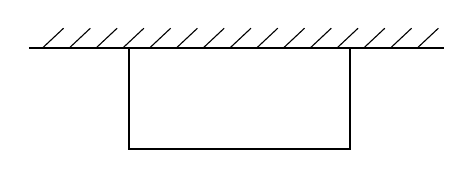
\begin{tikzpicture}[scale=0.85]
  \draw[thick] (-0.7,1.5) -- (5.5,1.5);
  \foreach \x in {-0.5,-0.1,...,5.1}
    \draw (\x,1.5) -- ++(0.32,0.3);
  \draw[thick] (0.8,1.5) -- (0.8,0) -- (4.1,0) -- (4.1,1.5);
\end{tikzpicture}
\end{center}
\nopagebreak[4]
\end{question}
\begin{question}
\gkti{8}\textbf{（14 分）} 已知：$\lg2=0.3010$，$\lg3=0.4771$。计算从 $1$ 到 $10$ 之间（除 $7$ 以外）所有整数的对数值。

\end{question}
\begin{question}
\gkti{9}\textbf{（12 分）} 已知顶点在原点的抛物线，关于 $y$ 轴对称，并且经过 $P(6,-2)$ 点。

（1） 求抛物线的方程；

（2） 画出它的大致图形；

（3） 写出它的焦点坐标和准线方程。

\end{question}
\begin{question}
\gkti{10}\textbf{（10 分）} 已知：$a$，$15$，$b$ 三个数成等差数列；$a$，$9$，$b$ 三个数成等比数列。求 $a$、$b$ 两个数。

\end{question}